\documentclass{beamer}
\include{darkbeamerthemes}
\usepackage{ragged2e}
\def\Z{\ensuremath\mathbb{Z}}
\def\C{\ensuremath\mathbb{C}}
\def\Q{\ensuremath\mathbb{Q}}
\def\N{\ensuremath\mathbb{N}} 
\def\R{\ensuremath\mathbb{R}}
\def\M{\ensuremath\mathcal{M}}
\def\N{\ensuremath\mathbb{N}}
\def\F{\ensuremath\mathbb{F}}
\setbeamertemplate{footline}[frame number]
\usepackage[linesnumbered,ruled,vlined]{algorithm2e}

\newcounter{saveenumi}
\newcommand{\seti}{\setcounter{saveenumi}{\value{enumi}}}
\newcommand{\conti}{\setcounter{enumi}{\value{saveenumi}}}
\newcommand{\fraka}{\ensuremath{\mathfrak{a}}}
\newcommand{\frakb}{\ensuremath{\mathfrak{b}}}
\usetheme{Hannover}
\usecolortheme{magpie}
%\usecolortheme{cormorant}
\title{Multivariate Multipoint Evaluation (MME)}
\author{Sarwagya Prasad, Rahul Bhardwaj}
\date{\today}

\AtBeginSection[]{
  \begin{frame}
  \vfill
  \centering
  \begin{beamercolorbox}[sep=8pt,center,shadow=true,rounded=true]{title}
    \usebeamerfont{title}\insertsectionhead\par%
  \end{beamercolorbox}
  \vfill
  \end{frame}
}

\begin{document}

\begin{frame}
\titlepage
\end{frame}

\begin{frame}{Content}
    \tableofcontents
\end{frame}
\section{Introduction}

\section{Univariate Multipoint Evaluation over Finite Fields}
\begin{frame}{Preliminaries 1}
    \begin{block}{Definition}
        Define the precision function for integers and polynomials as follows :
        \[\operatorname{prec}(U) = \begin{cases}\deg{U} + 1 & \text{if $U$ is a polynomial}, \\ \log_2 U & \text{if $U$ is an integer}.\end{cases}\]
    \end{block}

    \begin{block}{\textsc{PolyMult}}
        Multiplication of two polynomials of degree $n$ and $m$ takes : 
        \[\frac{9}{2} N \log{N} + 5N + \operatorname{ldt}\] time, where $N=n+m$.
    \end{block} 
\end{frame}
\begin{frame}{Preliminaries 2}
    \begin{block}{Divide and Rule}
        If the timing function of an algorithm satisfies the recurrence : 
        \[T(N) = 2T(N/2) + f(N)\],
        where $f(N) = \mathcal{O}(N\log^{a}(N))$, then $T(N) = \mathcal{O}(N\log^{a+1}(N))$.
    \end{block}
\end{frame}

\begin{frame}{Evaluation is Division}
    \begin{enumerate}
        \item Let $p(X) \in \mathbb{F}[X]$ be a polynomial which we want to evaluate at $x=\alpha \in \mathbb{F}$.
        \item By division algorithm, there exist $q(X), r(X)\in \mathbb{F}[X]$ such that $\deg{r}<\deg(x-\alpha)$: 
        \[p(X) = q(X)(x-\alpha) + r(x).\]
        \item Hence $p(\alpha) = r(\alpha)$, but since $\deg{r} = 0$, $r$ is a constant polynomial.
        \item Therefore, evaluating a polynomial at a point $\alpha$ becomes a problem of how quickly you can find the remainder of the corresponding division of the polynomial by $x-\alpha$.
    \end{enumerate}
\end{frame}

\begin{frame}{Evaluation is Division}
\justifying{
If we want to evaluate a polynomial $p(x)$ and $x_1,\ldots, x_N$, then we try to write $f(x) = q(x)\prod_{1\leq i\leq N} (x-x_i) + r(x)$, where $\def{r}<N$. Hence, $f(x_i) = r(x_i)$ for $1\leq i\leq N$. Therefore, we've reduced our problem to a simpler problem.It suffices to consider the problem of evaluating polynomials of degree $N-1$ on $N$ points. Let $M_1(x) = (x-x_1)\cdots(x-x_{N/2})$ and $M_2(x) = (x-x_{N/2+1})\cdots (x-x_N)$. We divide $p(x)$ by $M_1(x)$ to get $R_1(x)$ and by $M_2(x)$ to get $R_2(x)$. The problem now reduces to evaluating two polynomials of $N/2-1$ degree at $N/2$ points each.}
\end{frame}

\begin{frame}{Algorithm}
    Let $D$ be a Euclidean domain, we are given a set of $N$ moduli $\{m_i\}\in D$ and an element $U\in D$ for which we wish to compute the set of residues $u_i\in D$ such that : 
    \[u_i \equiv U \pmod{m_i}, \quad 1\leq i\leq N.\]

    \begin{block}{Theorem}
        \justifying{Given $N$ moduli $m_i\in D$ and $U\in D$ where $\operatorname{prec}(U)=N$, if multiplication and division of $N$ precision elements can be performed in $\mathcal{O}(N\log^a(N))$ operations, then the $N$ residues $\{u_i\}$ of $U$, with respect to $\{m_i\}$ can be computed in $\mathcal{O}(N\log^{a+1}(N))$ steps, where $a\geq 0$.}
    \end{block}
\end{frame}

\begin{frame}{Algorithm}

\boxed{\textsc{Modular Form}$(U,j,k)$}
\newline
\newline
\textbf{Input : } \begin{itemize}
    \item the requisite moduli $M_{jk}$,
    \item the element $U$ where $\operatorname{prec}(U)\leq k-j+1$.
\end{itemize}
\textbf{Output : } the residues $u_i \equiv U \bmod{m_i}, \quad j\leq i\leq k$.

\textbf{Step}
\begin{enumerate}
    \item If $j=k$, then output $U$ and go to step $4$.
    \item Let $e := \lfloor (j+k-1)/2\rfloor$ and $f := e+1$. Set $R_1 := U \operatorname{rem} M_{je}$ and $R_2 := U \operatorname{rem} M_{fk}$.
    \item Call $\textsc{Modular Forms}(R_1, j,e)$ and $\textsc{Modular Forms}(R_2, f,k)$.
    \item Return.
\end{enumerate}

\end{frame}

\section{Approximate Univariate Multipoint Evaluation over Complex}
\newcommand\blfootnote[1]{%
  \begingroup
  \renewcommand\thefootnote{}\footnote{#1}%
  \addtocounter{footnote}{-1}%
  \endgroup
}

\begin{frame}{Statement}
    \begin{block}{Problem Statement}
        Given a univariate polynomial $f \in \C[x]$ of degree d with $\lVert f \rVert \le 2^\tau$, and d points $x_1, x_2 \cdots x_d$ with absolute value less than 1, return the approximate evaluation of $f$ on these points, $y_1, y_2 \cdots y_k$ such that $\lvert f(x_i) - y_i \rvert \le \lVert f \rVert 2^{-m}$
    \end{block}
\end{frame}

\begin{frame}
    \frametitle{Nearly Linear Time}
    \begin{block}
        {Theorem}
        [Mor21]: The above problem can be solved in $\Tilde{O}\left(d (\tau + m)\right)$ bit operations.
    \end{block}

    \blfootnote{[Mor21]: Guillaume Moroz. New data structure for univariate polynomial approximation and appications in root isolation, numerical multipoint evaluation and other problems}
\end{frame}

\begin{frame}{Previous State of the Art}
    \begin{block}
        {Theorem}
        [KS16]: Let f be a polynomial of degree d, with $\Vert f \rVert_1 \le 2^\tau$, and let $x_1, x_2 \cdots x_d \in \C$ be complex points with absolute values bounded by 1. Then, computing $y_k$ such that $\lvert f(x_k) - y_k \rvert \le 2^{-m}$ is possible in $\Tilde{O}\left(d (m + \tau + d\right)$ bit operations.
    \end{block}    

    \blfootnote{[KS16]: Alexander Kobel and Michael Sagraloff. Fast approximate polynomial multipoint evaluation and many applications}
\end{frame}

\begin{frame}{Unit Disk Covering}
\begin{itemize}
    \item If $m < d$, the previous algorithm is optimal.
    \item If we had a m degree approximation of f, we could use the previous algorithm to get the required nearly linear time algorithm.
    \item However, we cannot hope a single m degree approximation to stay close to f. Thus we can make a \textbf{partition}, or more generally, a covering, of the unit disk with many small parts, and have approximations g for each small part such that g stays close to f in that region.
    \item Need to limit the number of parts, e.g., have $O \left(d / m \right)$ parts.
\end{itemize}
\end{frame}

\begin{frame}{N-Hyperbolic Covering}
    \begin{block}
        {Definition}
        [Mor21]: Given a positive integer N, an N-hyperbolic covering of the unit disk is the set of disks of centres $\gamma_n e^{2 \pi i \frac{k}{K_n}}$ and radii $\rho_n$, $0 \le n < N, 0 \le k < K_n$ where:
        \begin{align*}
            r_n &= \begin{cases}
                1 - \frac{1}{2^n} &, 0 \le n < N \\
                1 &, n = N
            \end{cases} \\
            \gamma_n &= \frac{1}{2}(r_n + r_{n+1}) \\
            \rho_n &= \frac{3}{4}(r_{n+1} - r_n) \\
            K_n &= \begin{cases}
                4 &, n = 0 \\
                \lceil \frac{3 \pi}{\sqrt{5}} \frac{r_{n+1}}{\rho_n} \rceil&, otherwise
            \end{cases}
        \end{align*}
    \end{block}
\end{frame}

\begin{frame}{Illustration of Hyperbolic Covering}
    \begin{figure}
        \centering
        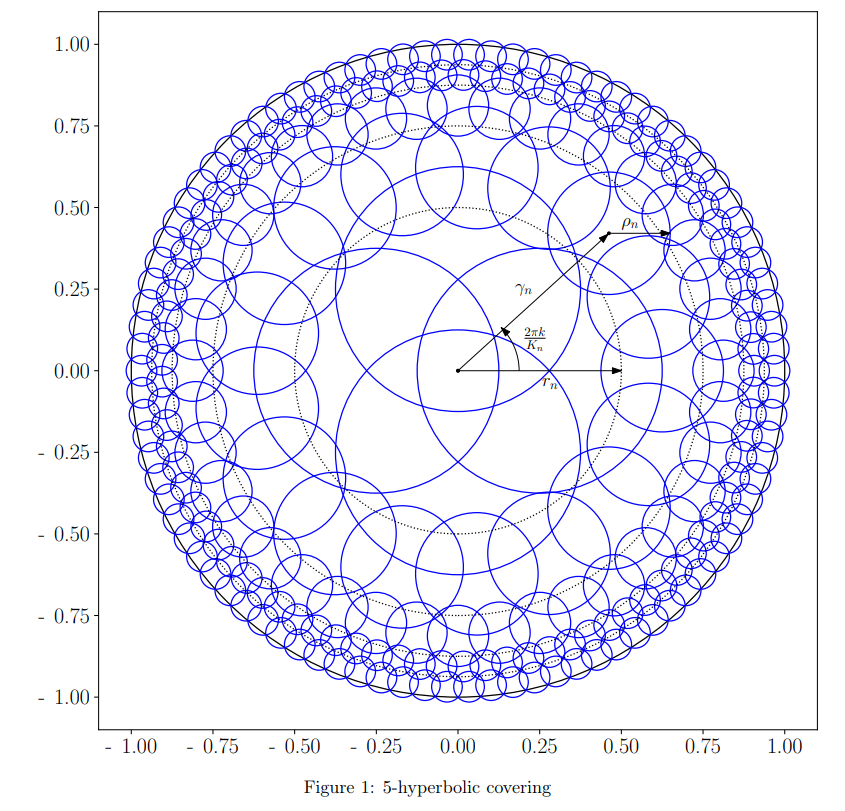
\includegraphics[scale=0.25]{Project Files/hyperbolic-cover.png}
        \label{fig:enter-label}
    \end{figure}
    % 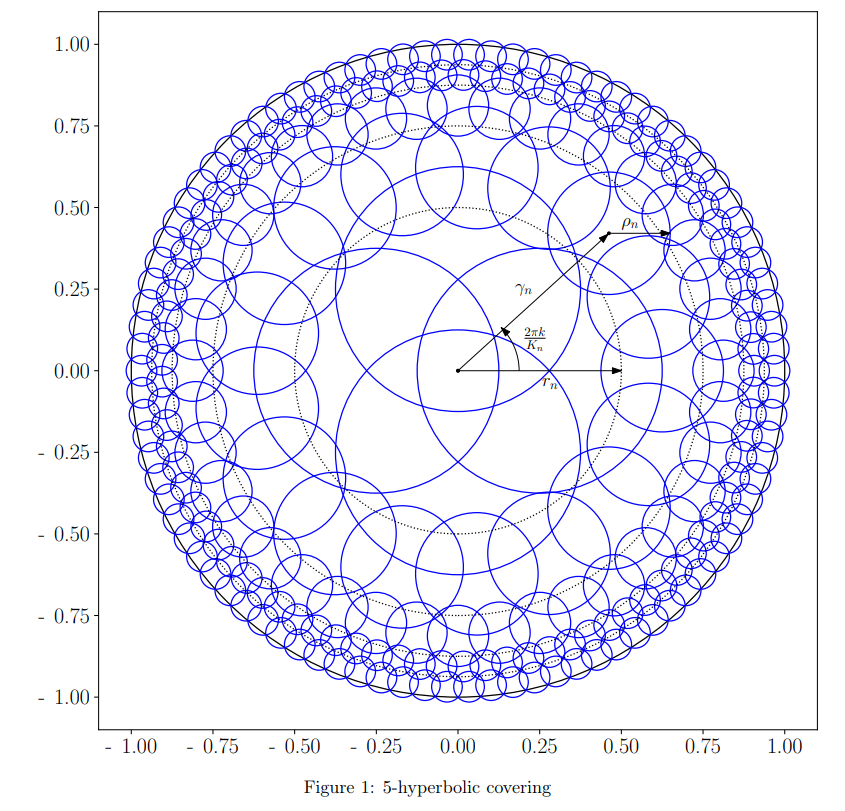
\includegraphics[scale=0.25]{Project Files/hyperbolic-cover.png}

    \blfootnote{[Mor21]}
\end{frame}

\begin{frame}{m-hyperbolic Approximation}
    Given a polynomial of degree d with $\lVert f \rVert \le 2^\tau$, and an integer $m > 1$, an m-hyperbolic approximation $H_{d, m}$ of f is a finite set of pairs $(g, a)$ where g is an m degree polynomial, and a is an affine transformation such that:
    \begin{itemize}
        \item The set of disks $a \left(D(0, 1)\right)$ is the N-hyperbolic covering, with $N = \lceil \log_2 \left(\frac{3ed}{m} \rceil \right)$, i.e., $a(X) = \left(\gamma_n + \rho_n X\right) e^{2 \pi i \frac{k}{K_n}}$
        \item $\lVert f \circ a - g \rVert \le 3 \lVert f \rVert 2^{-m}$
    \end{itemize}

    \blfootnote{[Mor21]}
\end{frame}

\begin{frame}{Number of disks}
    \begin{block}
        {Lemma} Given two integers d and $m > 1$, let $N = \lceil \log_2 \left(\frac{3ed}{m} \rceil \right)$. Then, the number of disks in the N-hyperbolic covering is in $O(d/m)$ and the union of the disks contains the unit disk.
    \end{block}

    \begin{block}
        {Proof}
        Total number of disks $t = \sum_0^{N-1}K_n$ \\
        We have $K_n \le 2^{n+4}$, $\Rightarrow t \le 2^{N=4} \le 16 \cdot 3e \frac{d}{m}$ \\
        Therefore, $t = O(d/m)$

        CLAIM: For any ring $R_n = D(0, r_{n+1}) \setminus D(0, r_n)$, the union of disks centered at $\gamma e^{2 \pi i \frac{k}{K_n}}$ with radius $\rho_n$ contains $R_n$.
    \end{block}

    \blfootnote{[Mor21]}
\end{frame}

\begin{frame}{Approximation Algorithm}
    \begin{block}
    {Theorem}
        Given a polynomial f of degree d, and an integer $ m > 1$, the m-hyperbolic approximation of f can be computed in $\Tilde{O}\left(d(m+\tau)\right)$
    \end{block}
\end{frame}

\begin{frame}{Approximation Algorithm}
    \begin{figure}
        \centering
        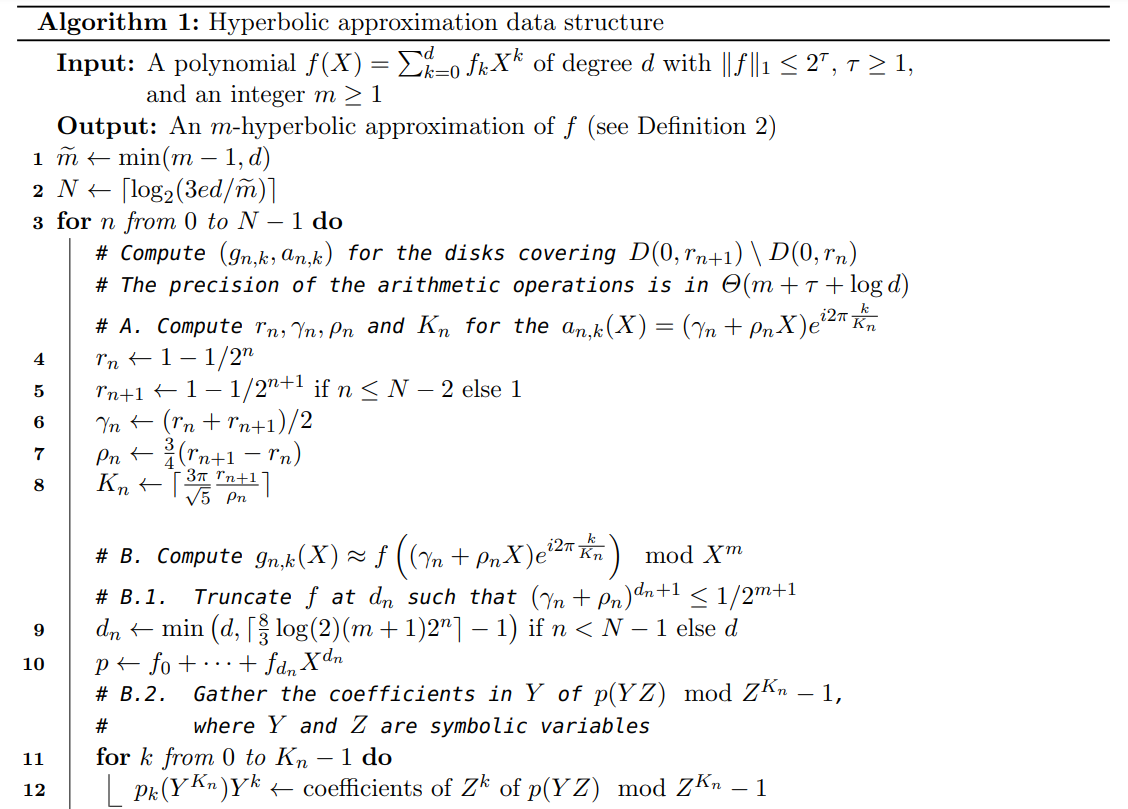
\includegraphics[scale=0.25]{Project Files/algo-1.png}
        \label{fig:enter-label}
    \end{figure}

    \blfootnote{[Mor21]}
\end{frame}

\begin{frame}{Approximation Algorithm}
    \begin{figure}
        \centering
        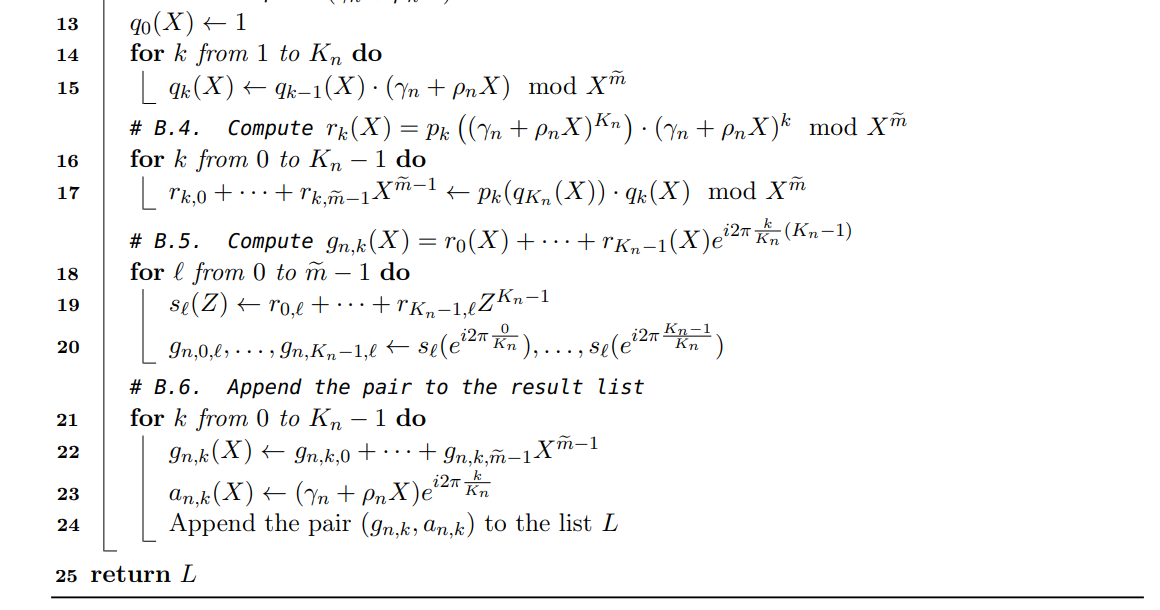
\includegraphics[scale=0.25]{Project Files/algo-2.png}
        \label{fig:enter-label}
    \end{figure}

    \blfootnote{[Mor21]}
\end{frame}

\begin{frame}{Overall Algorithm}
    \begin{algorithm}[H]
    \SetAlgoLined
    \KwData{polynomial f of degree d, d numbers $x_i \in D(0,1)$, precision m}
    \KwResult{List of evaluations $y_i$ such that $\lvert y_i - f(x_i) \rvert \le \lVert f \rVert 2^{-m}$}
        $L \leftarrow \{\}$ \\
        $Q \leftarrow$ data structure constructed from $x_i$, for fast disk range search \\
        $G \leftarrow H_{d, m+2}(f)$ \\

        \For{$(g_k, a_k)$ in G}{
        $v_1, \cdots v_{n_k} \leftarrow$ query Q for range $a_k$ \\
        $y_1, \cdots y_{n_k} \leftarrow g_k\left(a_k^{-1}(v_1)\right) \cdots g_k\left(a_k^{-1}(v_{n_k})\right)$ \\
        Append $y_1, \cdots y_k$ to L
        }
        \KwRet{$L$}\;
    \caption{\textsc{Approx-Multipoint-Eval} Algorithm}
\end{algorithm}
\end{frame}

\section{Multivariate Multipoint Evaluation over Finite Fields}
\newcommand\blfootnote[1]{%
  \begingroup
  \renewcommand\thefootnote{}\footnote{#1}%
  \addtocounter{footnote}{-1}%
  \endgroup
}


\begin{frame}{Preliminaries - CRT}
    \begin{block}
        {Lemma}
        \textbf{Fast CRT Modulation Computation [GG13]: } There is an algorithm that when given as input coprime positive integeres $p_1, \cdots p_r$ and a positive integer $N < \Pi p_i < 2^c$ computes the remainders $a_i \equiv N \text{ mod } p_i$ in $\Tilde{O}(c)$ time
    \end{block}

    \begin{block}
        {Lemma}
        \textbf{Fast CRT Reconstruction [GG13]: } There is an algorithm that when given input coprime positive integers $p_1, \cdots p_r$ and $a_1 \cdots a_r$ such that $0 \le a_i < p_i$ outputs the unique integer $0 \le N < \Pi p_i < 2^c$ such that $N \equiv a_i \text{ mod } p_i$ in $\Tilde{O}(c)$ time.
    \end{block}

    \blfootnote{[GG13]: Joachim Von Zur Gathen and Jurgen Gerhard: Modern Computer Algebra}
\end{frame}

\begin{frame}{Preliminaries - Kronecker Map}
    \begin{block}
        {Definition}
        \textbf{Kronecker Map: } The c-variate Kronecker Map for base-d denoted by $\Phi_{d,m;c}$ maps cm-variate polynomials into a c-variate polynomials via:
        \[
        \Phi_{d,m;c}\left(f(x_{11}, \cdots x_{1m}, \cdots x_{cm})\right) = f(1, y_1^d, y_1^{d^2} \cdots y_1^{d^{m-1}}, \cdots y_c^{d^{m-1}})
        \]
    \end{block}
\end{frame}

\begin{frame}{Frame Title}
    \begin{block}
    {Theorem}
        Given m-variate polynomial $f \in \F_p[x_1, \cdots x_m]$ with degree at most d-1 in each variable and $\alpha_1 \cdots \alpha_{N-1}$, then there exists a deterministic algorithm that outputs $f(\alph_i)$ in time: \[O\left(m(d^m + p^m + N) poly(\log p)\right)\]
    \end{block}

    \begin{block}
        {Proof}
        \begin{enumerate}
            \item Compute the reduction $\overline{f}$ of $f$ modulo $x_j^p - x$
            \item Use an FFT to compute $\overline{f}(\alpha)$ for all $\alpha \in \F_p^m$
            \item Look up and return $f(\alpha_i)$
        \end{enumerate}
    \end{block}
\end{frame}

\begin{frame}{MME Algorithm over Finite Fields}
    \tiny{\begin{algorithm}[H]
    \SetAlgoLined
    \KwData{$f(x_1,\ldots, x_n)\in\F_p[x_1,\ldots,x_n]$ and $\mathbf{a}^{(1)},\ldots, \mathbf{a}^{(N)}\in \F_p^N$}
    \KwResult{$b_i = f(\mathbf{a}^{(i)})$ for $i\in [N]$.}
        Adjust d and m such that $\log \log d \le m \le d^{o(1)}$
        Let $\Tilde{L} = (dm + 1) log p + m log d$. Compute first $\Tilde{L}$ prime numbers $\{p_1, \cdots p_{\Tilde{L}}\}$ \\
        Let $L\leq s$ be the smallest integer such that $p_1\cdots p_L =: M > d^m \cdot p^{dm+1}$ \\
        \For{$e\in \{0,\ldots, d-1\}^m$}{
            Compute $f_e^{(l)} = f_e \bmod{p_l}$ for $l\in L$.
        }
        \For{$i\in [N], k\in [m]$}{
            Compute $a_{i,k,l} = \mathbf{a}_k^{(l)}\bmod p_l$ for $l\in L$.
        }
        \For{$l\in [L]$}{
            Let $f^{(l)}(x_1,\ldots, x_m) = \sum_\mathbf{e}f_{\mathbf{e}}^{(l)}\mathbf{x}^{\mathbf{e}}\in \mathbb{F}_{p_l}[\mathbf{x}]$.\\
            Let $\mathbf{a}^{(i,l)}=(a_{i,1,l},\ldots, a_{i,m,l})\in \mathbb{F}_{p_l}^m$ for each $i\in [N]$.\\
            Compute $f_{(l)}(\alpha)$ for all $\alpha \in \F_p^m$ \\
            Look up and store $f^{(l)}(a^{(i, l)})$
        }
        \For{$i\in [N]$}
        {
            Compute the unique $b_i\in [-M/2, M/2]$ such that $b_i = b_{i,l} \bmod{p_l}$ for all $l\in [L]$.
        }
        \KwRet{$\{b_i : i\in [N]\}$}\;
    \caption{\textsc{MME-Finite-Field}}
\end{algorithm}}
\end{frame}


\section{Multivarate Multipoint Evaluation over Integers}
\begin{frame}{Exact-MME over $\Z$}
    \begin{block}{Problem Statement}
        \justifying{\textbf{Input : } An integer $s>0$, a polynomial $f(x_1,\ldots, x_n) \in \Z[x_1, \ldots, x_m]$ of individual degree less than $d$, given as a list of $d^m$ integer coefficients, a set of points $\mathbf{a}^{(1)},\ldots, \mathbf{a}^{(N)}\in \Z^m$ with each coordinate of magnitude at most $2^s$, with the guarantee that all coefficients of $f$, coordinates of $\mathbf{a}^{(i)}$'s, and evaluations $f(\mathbf{a}^{(i)})$ are bounded in magnitude by $2^s$.
\\  
        \textbf{Output : } Integers $b_1,\ldots, b_N$ that are the evaluations, i.e. $b_i = f(\mathbf{a}^{(i)})$ for $i\in [N]$.}
    \end{block}
\end{frame}

\begin{frame}{Exact-MME over $\Z$}
    \begin{block}{Theorem}
        There is a deterministic algorithm that on input as mentioned above returns the required output as mentioned above and runs in deterministic time $((d^m+Nm)\cdot s)^{1+o(1)}$ for all $m\in \N$ and sufficiently large $d\in \N$.
    \end{block}
\end{frame}

\begin{frame}{Algorithm}
    \tiny{\begin{algorithm}[H]
    \SetAlgoLined
    \KwData{$f(x_1,\ldots, x_n)\in\Z[x_1,\ldots,x_n]$ and $\mathbf{a}^{(1)},\ldots, \mathbf{a}^{(N)}\in \Z^N$, and an integer $s>0$ such that $|\mathbf{a}^{(i)}|<2^s$ and $|f(\mathbf{a}^{(i)})|<2^s$.}
    \KwResult{$b_i = f(\mathbf{a}^{(i)})$ for $i\in [N]$.}
        Compute the first $s$ prime numbers $\{p_1,\ldots, p_s\}$.\\
        Let $L\leq s$ be the smallest integer such that $p_1\cdots p_L =: M > 2^{s+1}$. \\
        \For{$e\in \{0,\ldots, d-1\}^m$}{
            Compute $f_e^{(l)} = f_e \bmod{p_l}$ for $l\in L$.
        }
        \For{$i\in [N], k\in [M]$}{
            Compute $a_{j,k,l} = \mathbf{a}_k^{(l)}\bmod p_l$ for $l\in L$.
        }
        \For{$l\in [L]$}{
            Let $f^{(l)}(x_1,\ldots, x_m) = \sum_\mathbf{e}f_{\mathbf{e}}^{(l)}\mathbf{x}^{\mathbf{e}}\in \mathbb{F}_{p_l}[\mathbf{x}]$.\\
            Let $\mathbf{a}^{(i,l)}=(a_{i,1,l},\ldots, a_{i,m,l})\in \mathbb{F}_{p_l}^m$ for each $i\in [N]$.\\
            Compute $b_{i,l} = f^{(l)}(\mathbf{a}^{(i,l)})$ for all $i\in [N]$ using Finite MME algorithm.
        }
        \For{$i\in [N]$}
        {
            Compute the unique $b_i\in [-M/2, M/2]$ such that $b_i = b_{i,l} \bmod{p_l}$ for all $l\in [L]$.
        }
        \KwRet{$\{b_i : i\in [N]\}$}\;
    \caption{\textsc{Exact-MME-Integers}}
\end{algorithm}}
\end{frame}
\end{document}